\section{Proposed Methods}
\label{sec:methods}

\subsection{The DeepLab CNN + CRF Model for Semantic Image Segmentation}

Our starting point is the recently proposed DeepLab model for semantic
image segmentation of \citet{chen2014semantic}, illustrated in
Figure~\ref{fig:model_test}. This model applies a deep CNN to an image
in a sliding window fashion to generate score maps for each pixel
location $i = 1, \dots, N$
\begin{equation}
  \label{eq:scores}
  f_i(x; \theta) \,,
  \quad \mathrm{with} \quad
  P_i(x; \theta) \propto \exp \left( f_i(x; \theta) \right)
\end{equation}
where $x \in \mathcal{L}$ is the assignment to the discrete candidate
semantic label set $\mathcal{L}$, $\theta$ is the vector of CNN model
parameters, and normalization ensures that $\sum_{x \in  \mathcal{L}}
P_i(x; \theta) = 1$ for every pixel $i$. Score map post-processing by
means of a fully-connected CRF (Dense CRF)
\cite{krahenbuhl2011efficient} significantly improves segmentation
performance near object boundaries. Computation sharing in the
convolutional layers by means of the hole algorithm and careful
network crafting as detailed in \citet{chen2014semantic} make the
method computationally efficient.

\begin{figure}[htbp!]
  \centering
  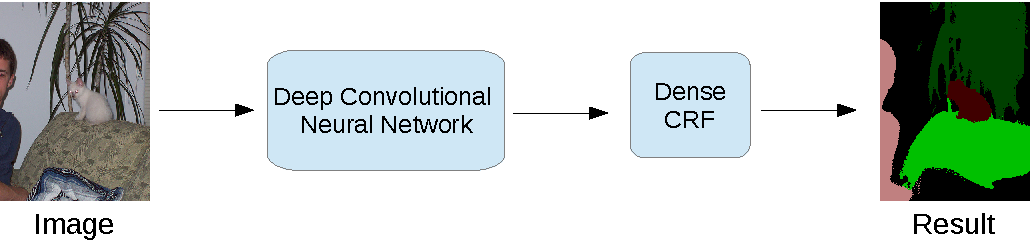
\includegraphics[width=0.9\linewidth]{fig/model_test.pdf} 
  \caption{Overview of the DeepLab CNN + CRF semantic segmentation model.}
  \label{fig:model_test}
\end{figure}

\subsection{Model Training on Fully Annotated Images}
\label{sec:train_pixel}

The network parameters $\theta$ are initialized from an
Imagenet-pretrained deep CNN model \citep{simonyan2014very} and
fine-tuned by stochastic gradient descent so as to minimize the
average log-loss 
\begin{equation}
  \label{eq:log_loss}
  L(\theta) = \frac{1}{N} \sum_{i = 1}^N \log P_i(l_i; \theta)
\end{equation}
between the model predictions and the pixel-wise ground truth
labels $\{l_i\}_{i = 1}^N$, as illustrated in
Figure~\ref{fig:model_train_pixel}. Similarly to
\citet{chen2014semantic}, we do not include the Dense CRF module into
the training pipeline for simplicity and speed during training.

Learning the DeepLab model on fully annotated images works very well
in practice, yielding excellent performance (66.4 \% IoU) in the
challenging PASCAL VOC 2012 image segmentation benchmark. However, the
need for such detailed annotations makes it harder to gather very
large training datasets and makes it difficult to train the model
for new domains, especially when the number of candidate labels
(\ie, the cardinality of the label set $\mathcal{L}$) is large.

\begin{figure}[htbp!]
  \centering
  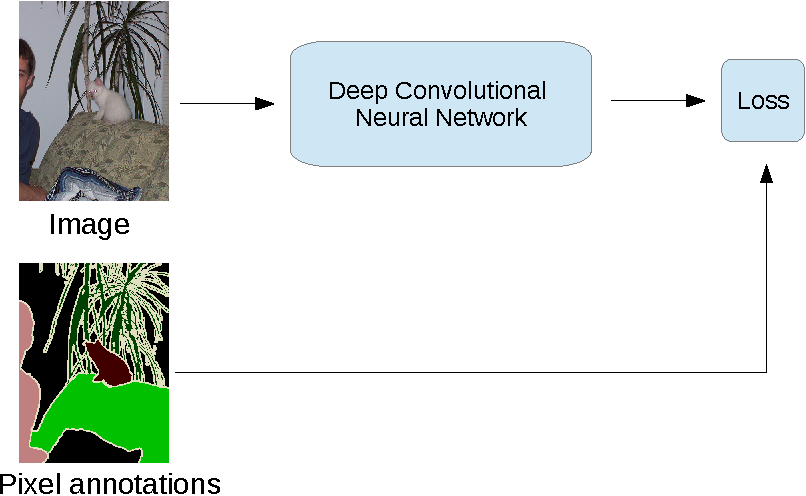
\includegraphics[width=0.9\linewidth]{fig/model_train_pixel.pdf} 
  \caption{DeepLab model training from fully annotated images.}
  \label{fig:model_train_pixel}
\end{figure}

\subsection{Model Training on Weak Bounding Box Annotated Images}
\label{sec:train_bbox}

Collecting bounding box annotations is significantly easier compared
to pixel-level ground truth segmentations. We have explored two
methods for training the DeepLab segmentation model from bounding
boxes with object-level labels. In both methods we estimate dense
segmentation maps from the bounding box annotation as a pre-processing
step, then employ the training procedure of
Section~\ref{sec:train_pixel} treating these estimated labels as
ground-truth.

The first baseline method amounts to simply considering each pixel
within the bounding box as positive example for the respective object
class. Ambiguities are resolved by assigning pixels that belong to
multiple bounding boxes to the one that has the smallest area.

\emph{GRABCUT GOES HERE}

\begin{figure}[htbp!]
  \centering
  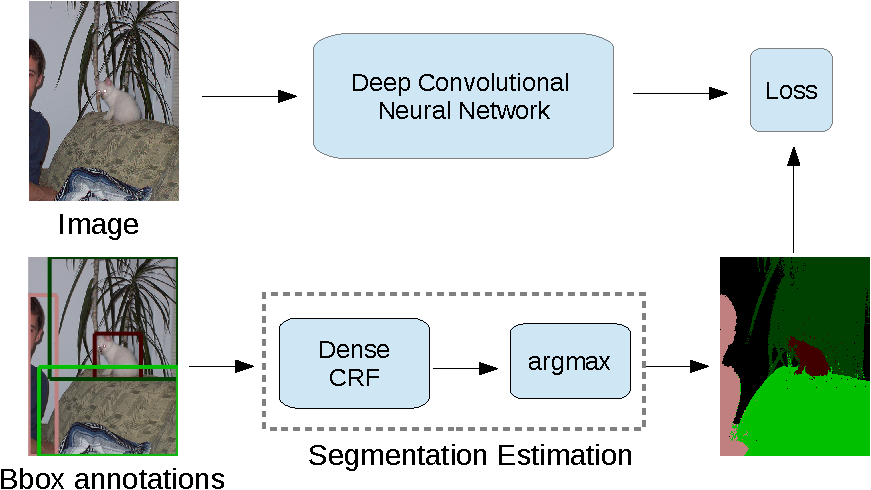
\includegraphics[width=0.9\linewidth]{fig/model_train_bbox.pdf} 
  \caption{DeepLab model training using bounding box data and
    automated foreground/ background segmentation.}
  \label{fig:model_train_bbox}
\end{figure}


\subsection{Model Training Using Weak Image-Level Labels}

Training the DeepLab segmentation model using only image-level labels
is significantly more challenging.

\paragraph{Previous MIL Approaches and their Limitations}

Previous related CNN literature employs multiple instance learning
variants to address the weak supervision problem, but has demonstrated
limited success in learning accurate segmentation models. 

In particular, recent work by \citet{pathak2014fully} attempts to
learn the CNN parameters for the segmentation model by adapting an MIL
formulation previously employed for image classification tasks
\citep{oquab2014weakly, papandreou2014untangling}. More specifically,
during training they compute an aggregate image-level response for
each class $x$ as the maximum class score across all pixel positions
$i$
\begin{equation}
  \label{eq:mil}
  \bar{f}(x; \theta) = \max_i f_i(x; \theta) \,
  \quad \mathrm{and} \quad
  \bar{P}(x; \theta) \propto \exp \left( \bar{f}(x; \theta) \right)
\end{equation}
which is then combined with the image-level ground-truth label $l$ to
compute the whole-image loss $\bar{L}(\theta) = \log \bar{P}(l;
\theta)$.

There are several limitations to this MIL-based approach to the image
segmentation problem. \emph{First}, the model does not explicitly
encourage good localization during training, since it suffices to give
strong response for the correct class anywhere within the
image. \emph{Second}, this MIL formulation does not promote good
object coverage. For example, it is often sufficient to learn a good
face detector to reliably determine whether an image contains a
person. However, this face detector will give low false-negative
responses on the rest of the human body and is thus not appropriate
for segmenting whole persons. \emph{Third}, network back-propagation
only activates a single path per label through the maximally
responding pixel position ignoring a large portion of the image
content, thus slowing down training. These issues have severely
undermined the success of previous CNN/MIL approaches to image
segmentation and the performance of such models trained on weak labels
significantly lags their counterparts trained on pixel-level
annotations, as explained in Section~\ref{sec:experiments}.

\paragraph{Adapting Expectation-Maximization for Weakly-Labeled Training}

We propose an alternative training procedure based on a modified
Expectation-Maximization (EM) algorithm adapted to our weakly-labeled
image segmentation setting.

In this setting, we consider the pixel-level semantic labels
$\{l_i\}_{i=1}^N$ as latent variables. We incorporate the image-level
semantic labels as side-information that biases the E-step of the EM
algorithm, as detailed in Algorithm~\ref{algo:em_fixed_bias} and
illustrated in Figure~\ref{fig:model_train_image}. The positive
foreground and background biases $c_f$ and $c_b$ favor the score maps
corresponding to labels present in the image according to the
image-level weak annotation, similarly to \cite{Lu2013sports}. We have
obtained better results by choosing $c_f > c_b$, slightly favoring
foreground objects over the background.

\begin{algorithm}[!htbp]
  \centering
  \begin{algorithmic}[1]
    \algrenewcommand\algorithmicrequire{\textbf{Input:}}
    \Require CNN parameters $\theta$ and biases $c_f, c_b > 0$.
    \algrenewcommand\algorithmicrequire{\textbf{E-Step:}}
    \Require For each image position $i$
    \State $\hat{f}_i (x; \theta) = f_i(x; \theta) + c_f$, if label $x$ present \Comment{FG bias}
    \State $\hat{f}_i (x; \theta) = f_i(x; \theta) + c_b$, if $x$ is BG label \Comment{BG bias}
    \State $\hat{f}_i (x; \theta) = f_i(x; \theta)$, if label $x$ not present
    \State $\hat{l}_i = \argmax_i \hat{f}_i (x; \theta)$ \Comment{Hard assignments}
    \algrenewcommand\algorithmicrequire{\textbf{M-Step:}}
    \Require
    \State $\hat{L}(\theta) = \frac{1}{N} \sum_{i = 1}^N \log P_i(\hat{l}_i; \theta)$ \Comment{Expected loss}
    \State Update $\theta$ by SGD with momentum on $\hat{L}(\theta)$
    \end{algorithmic}
  \caption{Weakly-Supervised EM (fixed bias version)}
  \label{algo:em_fixed_bias}
\end{algorithm}

\begin{figure}[htbp!]
  \centering
  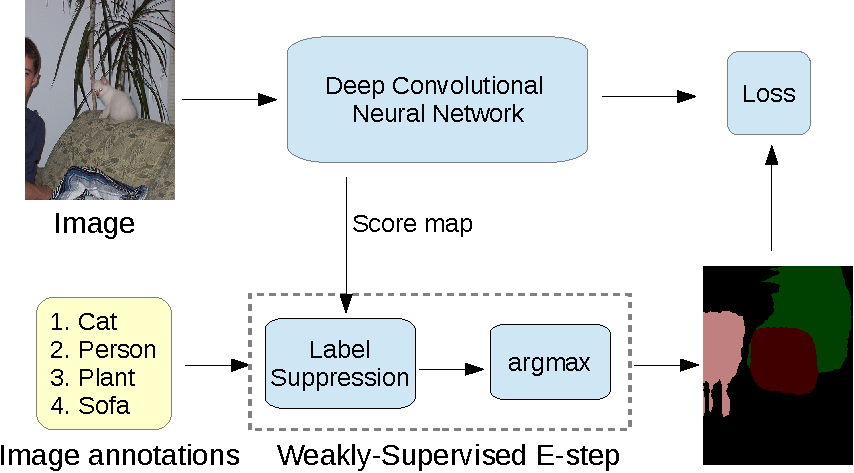
\includegraphics[width=0.9\linewidth]{fig/model_train_image.pdf} 
  \caption{DeepLab model training using image-level labels by
    biased Expectation-Maximization.}
  \label{fig:model_train_image}
\end{figure}

We have also experimented with an adaptive variant of
Algorithm~\ref{algo:em_fixed_bias} in which the biases are chosen
adaptively per image so as a pre-defined proportion of the image area
is assigned to the foreground object class, similarly to
\citet{kuck2005individuals}. This acts as a hard constraint that
explicitly prevents the background score from prevailing in the whole
image. As reported in the experimental section, we have found this
adaptive variant to perform better in the purely weakly supervised
scenario, whereas the fixed bias variant works best in the presense of
both weak and strong annotations discussed next.

\subsection{Model Training with a Combination of Fully and Weakly Annotated Images}

In practice, we often have access to a large number of weakly
image-level annotated images and can only afford to procure detailed
pixel-level annotations for a small fraction of these images. We
propose to handle this hybrid training scenario by combining the
methods presented in the previous sections, as illustrated in
Figure~\ref{fig:model_illustrations_twoEnd}. In SGD training of our
deep CNN models, we bundle to each mini-batch a fixed proportion of
strongly/ weakly annotated images, and employ our fixed-bias EM
algorithm in estimating at each iteration the latent semantic
segmentations for the weakly annotated images. We demonstrate in
Section~\ref{sec:experiments} that one needs to annotate in detail at
the pixel-level only a small part of the dataset and use image-level
labels for the remaining part to achieve the same level of performance
with a DeepLab model trained with the whole dataset fully annotated.

\begin{figure}[htbp!]
  \centering
  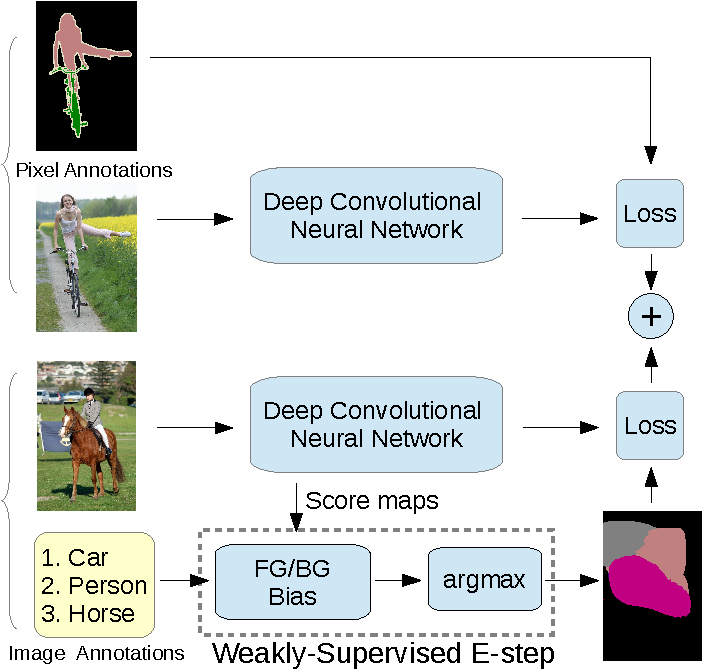
\includegraphics[width=0.9\linewidth]{fig/model_train_twoEnd.pdf} 
  \caption{DeepLab model training on a union of full (strong labels) 
    and image-level (weak labels) annotations.}
  \label{fig:model_illustrations_twoEnd}
\end{figure}

\subsection{Exploiting Annotations Across Datasets}

Finally, we discuss how we can exploit annotations across different
datasets potentially having different label spaces, also allowing for
the possibility annotations to be in part weak and in part strong. For
concreteness, consider leveraging the 81-label MS COCO dataset in
learning the DeepLab model for 21-label Pascal VOC 2012
segmentation. We have experimented with the following scenarios:
\begin{enumerate}
\item Pre-train DeepLab on MS-COCO, then replace the top-level
  classifiers weights and fine-tune on Pascal VOC 2012, using strong
  labels in both datasets.
\item Jointly train DeepLab on MS-COCO and Pascal VOC 2012 sharing
  the top-level classifier weights for the common classes, using
  strong labels in both datasets.
\item Jointly train DeepLab on MS-COCO and Pascal VOC 2012 sharing
  the top-level classifier weights for the common classes, using a
  combination of strong and weak labels.
\end{enumerate}

 %%% Local Variables:
 %%% mode: latex
 %%% TeX-master: "top.tex"
 %%% End:
